\documentclass[main.tex]{subfiles}


\begin{document}
\linenumbers

  

\chapter[Atomic structure]{Atomic structure}
%\label{ch:atoms}

\begin{marginfigure}
      \includegraphics{chapter3/figure1}
      \label{fig:marginfig1}
   \end{marginfigure}
\lettrine[lines=4]{\color{black!45}M}{atter} is everywhere around you, from the water you drink to the air you inhale. Matter is made of elements and elements are made of atoms. In the world we can also find light, that somehow at first sight seems different than matter. Light is warm and it has color. This chapter covers the structure of the atoms, with a focus on the structure of the many electrons than atoms are made of. It also focuses on light and the interaction of light with matter. You will be able to understand differences in electronic configuration.
 
\begin{marginfigure}%LEARNING GOALS BOX
\begin{mytcbox}{GOALS}
\begin{enumerate}[label=\protect\circled{\color{white}\arabic*}]
\item Compute frequency, wavelength and the energy of light
\item Compute energy the levels for \ce{H}
\item Compute transition energies for \ce{H}
\item Obtain electronic configurations
\item Compare periodic properties
\end{enumerate}
\end{mytcbox}
\end{marginfigure}%LEARNING GOALS BOX



\section{Light}
What is light? Light--also called electromagnetic radiation--is a form or energy. There are many different types of radiation. Think about the light coming from a bulb, or the radiation that warms up your food in a microwave, or even when you heat a pizza in the over. Radiation is characterized by frequency and by the wavelength. This section will cover these two properties of light.
  \begin{marginfigure}
\begin{tcolorbox}[enhanced,colback=red!5!white,colframe=black!50!red,boxrule=1pt,
  arc=0pt,outer arc=0pt,drop heavy lifted shadow]
\faGears\ 
\docenvdef{Discussion:} Look around your apartment and find four different types of radiation.\end{tcolorbox}
 \end{marginfigure}
\sloppy
\begin{description}
\item[\docfilehook{Frequency and energy}{Frequency and energy}] Light travels in time. That is the reason you can hear a whistle from afar. The \emph{frequency} of a radiation--the frequency of a specific type of light--characterizes how this radiation oscilates in time. The unit of frequency is the hertz and frequency is represented by the symbol $\gamma$. At the same time, frequency is connected to the energy of radiation. High frequency radiation are very energetic. Think for example of gamma rays; these type of radiation produced in nuclear plant has very high frequency and hence is very energetic. The formula that related frequency with energy is:\resizeableyellownote{2.5}{1}{Add this formula to your flashcard.}
\begin{equation*}
\boxed{  E=6.6\times 10^{-34}\gamma  } \quad \textcolor{blue}{\text{Frequency formula}}
\end{equation*}
where:
\begin{where}
 \item $E$   is the energy in joules
  \item $6.6\times 10^{-34}$ is called Plank's constant, $h$
 \item $\gamma$  is frequency in hertzs (Hz)
\end{where}
As you can see in the previous formula, the frequency is directly proportional to frequency.
\item[\docfilehook{Wavelength and energy}{Wavelength and energy}] Light also travels in space. As it moves, it oscillates in space. Think about dropping a stone into a lake. As you drop the pebble, the energy from the pebble propagates in the surface in water. The energy of light also propagates in space and the \emph{wavelength} of a radiation is the distance between two consecutive peaks. As such, wavelength, represented by the letter $\lambda$ and with units of $nm$ is also related to energy by means of the formula:
\resizeableyellownote{2.5}{1}{Add this formula to your flashcard.}
\begin{equation*}
\boxed{  E=\frac{1.98\times 10^{-16}}{\lambda}  } \quad \textcolor{blue}{\text{wavelength formula}}
\end{equation*}
where:
\begin{where}
 \item $E$   is the energy in joules
 \item $\lambda$  is wavelength in $nm$
  \item $1.98\times 10^{-16}=h\cdot c\cdot 10^{9}$  was adjusted to be able to use $\lambda$ in nm
\end{where}
Mind that wavelength is inversely related to energy. That means, the larger wavelength the smaller energy. Also mind that wavelength refers to the movement of light in space and frequency refers to the movement in time.

\item[\docfilehook{Relationship between wavelength and frequency}{Relationship between wavelength and frequency}] 
Wavelength and frequency are related by means of the speed of light $c$ that is $3\times 10^8$. However, if we want $\lambda$ to be in nm we can use the following formula:
\resizeableyellownote{2.5}{1}{Add this formula to your flashcard.}
\begin{equation*}
\boxed{  \gamma=\frac{3\times 10^{17}}{\lambda}  } 
\end{equation*}
where:
\begin{where}
 \item $\gamma$   is frequency in Hz
 \item $\lambda$  is wavelength in $nm$
  \item $3\times 10^{17}=c\cdot 10^{9}$   was adjusted to be able to use $\lambda$ in nm

\end{where}
All radiation always travels at the speed of light. At the same time, this speed is the maximum speed allowed for any object.



\begin{marginfigure}[0cm]
      \includegraphics{chapter3/figure1-1}
      \caption{White light contains many colors.}
      \label{fig:marginfig2}
   \end{marginfigure}
   
   
   \begin{marginfigure}[0cm]
     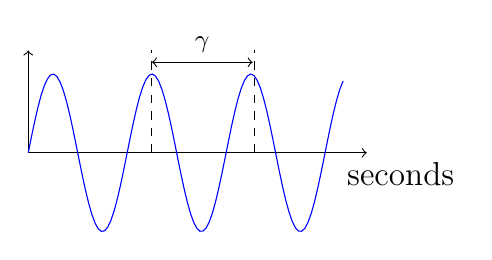
\begin{tikzpicture}[xscale=1,yscale=1]
  \draw[->] (0,0) -- (0,1.3);
  \draw[->] (0,0)--(4.3,0) node[font=\large,black, below, pos = 1.1] {seconds};
  \draw[domain=0:4,samples=100,blue] plot(\x,{sin(\x r*5)});
  \draw[dashed] (pi/2,0) -- (pi/2,1.3);
  \draw[dashed] (pi/2+1.3,0) -- (pi/2+1.3,1.3);
  \draw[<->] (pi/2,1.15) -- node[above]{\small $\gamma$} (pi/2+1.28,1.15);
\end{tikzpicture}
      \caption{Frequency refers to time}
   \end{marginfigure}
   
   
      \begin{marginfigure}[0cm]
     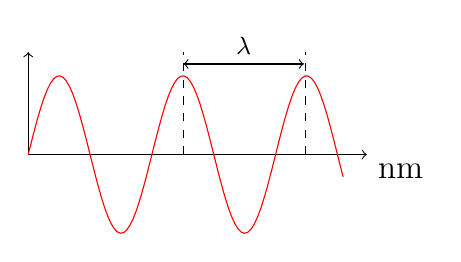
\begin{tikzpicture}[xscale=1,yscale=1]
  \draw[->] (0,0) -- (0,1.3);
  \draw[->] (0,0)--(4.3,0) node[font=\large,black, below, pos = 1.1] {nm};
  \draw[domain=0:4,samples=100,red] plot(\x,{sin(\x r*4)});
  \draw[dashed] (pi/2+0.4,0) -- (pi/2+0.4,1.3);
  \draw[dashed] (pi/2+0.65+1.3,0) -- (pi/2+0.65+1.3,1.3);
  \draw[<->] (pi/2+0.4,1.15) -- node[above]{\small $\lambda$} (pi/2+0.65+1.28,1.15);
\end{tikzpicture}
      \caption{Wavelength refers to space}
   \end{marginfigure}
   
   
   
   
\begin{example} %%%%%%%%%%%%%%%%%%%%%%%% EXAMPLE BOX
Calculate: (a) the energy of a radiation with wavelength of 300nm; (b) the energy of a radiation with frequency of $10^{19}$ Hz; (c) the frequency of a radiation with wavelength of 300nm.\\
\textlcsc{ \textcolor{dgreen}{\Large \textbf{Solution}} }\\
(a) To answer the first question we will use the wavelength formula, as wavelength is given ($\lambda=300nm$) and we need to calculate the energy ($E$), in Joules:
\begin{equation*}
E=\frac{1.98\times 10^{-16}}{\lambda}=\frac{1.98\times 10^{-16}}{300}=6.6\times 10^{-19}J
\end{equation*}
(b) To answer the second question we will use the frequency formula, as frequency is given ($\gamma=10^{19}Hz$) and we need to calculate the energy ($E$), in Joules:
\begin{equation*}
E=6.6\times 10^{-34}\gamma=6.6\times 10^{-34}\cdot 10^{19}=6.6\times 10^{-15}J
\end{equation*}
(c) To answer the last question we will use the formula that related frequency with wavelength--through the speed of light--as frequency is asked and wavelength is given ($\lambda=300nm$); mind the units of frequency are herts:
\begin{equation*}
\gamma=\frac{3\times 10^{17}}{\lambda}=  \frac{3\times 10^{17}}{300}=1\times 10^{15}Hz
\end{equation*}
\faDiamond\ \textlcsc{ \textcolor{dgreen}{\Large \textbf{Study Check}} }\\
Calculate: (a) the wavelength of radiation with energy of $5.6\times 10^{-19}J$; (b) the frequency of a radiation with frequency of $4.8\times 10^{-18}J$; (c) the wavelength of a radiation with frequency of $2\times 10^{15}Hz$.
\flushright Answer: (a) $353nm$; (b) $7.2\times 10^{10}Hz$; (c) $4.1\times 10^{6}nm$
\end{example}%%%%%%%%%%%%%%%%%%%%%%%% EXAMPLE BOX

\begin{marginfigure}[-2cm]%%%%%%%MARGIN FIGURE
\begin{tcolorbox}[tab2,tabularx={>{\hsize=.4\hsize}X|X}]%%%% FANCY COLOR TABLE
 Radiation     &  $\gamma$ (Hz)          \\\hline\hline
Gamma  &   \small >$3\times 10^{19}$        \\\hline
X-rays  &   \small $3\times 10^{19}-3\times 10^{16}$        \\\hline
UV  &   \small $3\times 10^{16}-8\times 10^{14}$        \\\hline
IR  &   \small $4\times 10^{14}-4\times 10^{11}$        \\\hline
MicroW &   \small $3\times 10^{11}-3\times 10^{8}$        \\\hline
RadioW  &   \small $3\times 10^{8}-3\times 10^{3}$                     
\end{tcolorbox}%%%% FANCY COLOR TABLE
 \end{marginfigure}%%%%%%%MARGIN FIGURE





\item[\docfilehook{Types of radiation}{Types of radiation}] 
Depending on its frequency--or on its wavelength--radiation can be classified as gamma rays, x rays, ultraviolet (UV), visible, infrared (IR), microwaves or radiowaves.
 \begin{figure}%%%%%%%MARGIN FIGURE
\tikzstyle{every picture}+=[remember picture]
\tikzstyle{na} = [baseline=-.5ex]
\begin{tikzpicture}[fill between/on layer={axis grid}, line width=1pt]
\begin{axis}[
legend columns=-1,
xlabel={Wavelength},
xticklabel style = {font=\tiny,yshift=0.2ex},
minor tick style={draw=none},
xmin=10^-4,
xmax=10^12	,
xtick distance=10^2,
xticklabel pos=top,
x unit=\si{\nano\meter},
xmode=log,
ymin=0,
ymax=1,
major tick length=1.5cm,
height=3cm,
yticklabels={},
ytick=\empty,
legend cell align=left,
legend style={at={(0.85,3.77)},anchor=north}
]
\addplot[draw=none, name path=start, forget plot] coordinates{(10^-4,0)(10^-4,1)} ;
\addplot[draw=none, name path=gamma, forget plot] coordinates{(10^-3,0)(10^-3,1)} node[font=\tiny,white, above, sloped, pos = .5] {Gamma Rays};
\addplot[draw=none, name path=xrays, forget plot] coordinates{(10^-1,0)(10^-1,1)} node[font=\tiny,white, above, sloped, pos = .5] {X-Rays};
\addplot[draw=none, name path=uv, forget plot] coordinates{(400,0)(400,1)} ;
\addplot[draw=none, name path=visible, forget plot] coordinates{(700,0)(700,1)};
\addplot[draw=none, name path=ir, forget plot] coordinates{(10^1,0)(10^1,1)} node[font=\tiny,white, above, sloped, pos = .5] {UV};
\addplot[draw=none,  forget plot] coordinates{(10^4,0)(10^4,1)} node[font=\tiny,white, above, sloped, pos = .5] {IR};
\addplot[draw=none,  forget plot] coordinates{(10^7,0)(10^7,1)} node[font=\tiny,white, above, sloped, pos = .5] {Microwaves};
\addplot[draw=none,  forget plot] coordinates{(10^11,0)(10^11,1)} node[font=\tiny,white, above, sloped, pos = .5] {Radiowaves};
\addplot[draw=none, name path=radiowave, forget plot] coordinates{(10^12,0)(10^12,1)};
\addplot[back, area legend] fill between[of=start and uv];
%\addlegendentry{$\gamma$-ray}
%\addplot[black, area legend] fill between[of=gamma and xrays];
%%\addlegendentry{X-ray}
%\addplot[black, area legend] fill between[of=xrays and uv];
%%\addlegendentry{Ultra violet}
\addplot[shading=visiblelight, area legend] fill between[of=uv and visible];
%%\addlegendentry{Visible light}
%\addplot[black, area legend] fill between[of=visible and ir];
%%\addlegendentry{Infrared}
%\addplot[black, area legend] fill between[of=ir and microwave];
%%\addlegendentry{Micro wave}
\addplot[black, area legend] fill between[of=visible and radiowave];
%\addlegendentry{Radio wave}
\end{axis}


\end{tikzpicture}
\begin{tikzpicture}[overlay]
\draw [thin, black, dotted]  (-6.26,0.09) -- ++(-4.30,-0.81) ;
\draw [thin, black, dotted]  (-6.30,0.09) -- ++(2.9,-0.81) ;
\end{tikzpicture}


\vspace{0.5cm}
\begin{tikzpicture}[x={(100.25,0)}, xshift=6cm]
\begin{axis}[
at={(-1cm,-3cm)},
xlabel={Visible wavelength},width=250pt,
xticklabel style = {font=\tiny,yshift=0.2ex},
minor tick style={draw=none},
xmin=400,
xmax=700,
x unit=\si{\nano\meter},
ymin=0,
ymax=1,
major tick length=1.5cm,
height=3cm,
yticklabels={},
ytick=\empty,
legend cell align=left,
legend style={at={(0.85,-2.77)},anchor=north}
]
\addplot[draw=none, name path=start, forget plot] coordinates{(400,0)(400,1)};
\addplot[draw=none, name path=a, forget plot] coordinates{(380,0)(380,1)};
\addplot[draw=none, name path=b, forget plot] coordinates{(435,0)(435,1)};
\addplot[draw=none, name path=c, forget plot] coordinates{(500,0)(500,1)};
\addplot[draw=none, name path=d, forget plot] coordinates{(520,0)(520,1)};
\addplot[draw=none, name path=e, forget plot] coordinates{(565,0)(565,1)};
\addplot[draw=none, name path=f, forget plot] coordinates{(590,0)(590,1)};
\addplot[draw=none, name path=g, forget plot] coordinates{(625,0)(625,1)};
\addplot[draw=none, name path=h, forget plot] coordinates{(700,0)(700,1)};
\addplot[violet, area legend] fill between[of=a and b];
\addplot[blue, area legend] fill between[of=b and c];
\addplot[cyan, area legend] fill between[of=c and d];
\addplot[green, area legend] fill between[of=d and e];
\addplot[yellow, area legend] fill between[of=e and f];
\addplot[orange, area legend] fill between[of=f and g];
\addplot[red, area legend] fill between[of=g and h];
\end{axis}
\end{tikzpicture}
    \caption{Spectrum of the electromagnetic radiation}   
 \end{figure}%%%%%%%MARGIN FIGURE



\begin{marginfigure}[4cm]%%%%%%%MARGIN FIGURE
\begin{tcolorbox}[tab2,tabularx={X|X}]%%%% FANCY COLOR TABLE
 Color     &  $\lambda$ (nm)          \\\hline\hline
Violet  &   \small 380-450       \\\hline
Blue  &   \small 450-485         \\\hline
Cyan  &   \small 485-500        \\\hline
Green &    \small 500-565      \\\hline
Yellow &    \small 565-590        \\\hline
Orange  &   \small 590-625   \\\hline     
Red  &   \small 625-740                               
\end{tcolorbox}%%%% FANCY COLOR TABLE

 \end{marginfigure}%%%%%%%MARGIN FIGURE




For example, radiation with wavelength of $10^{-2}$ nm belongs to gamma rays radiation, whereas radiation with wavelength of $10^{4}$ nm belongs to the Infrared. Only a small range of wavelengths belong to visible radiation. This means you will not be able to see IR radiation. The color of the radiation is also dependent on the wavelength--of the frequency as both are related--and for example $\lambda=450$ nm will be blue light.
\begin{example} %%%%%%%%%%%%%%%%%%%%%%%% EXAMPLE BOX
Indicate: (a) the color of a radiation with $\lambda=650nm$; (b) the type of a radiation with  $\lambda=10^{5}$ nm; (c) the type of a radiation with  $\gamma=10^{16}$ Hz.\\
\textlcsc{ \textcolor{dgreen}{\Large \textbf{Solution}} }\\
We can answer the first questions by inspecting the figure above we can see that $\lambda=650nm$ corresponds to red radiation. To answer the second question we will also use the figure above, where we can see that $\lambda=10^{5}$ nm belongs to the infrared. Finally, in order to answer the last question we need to convert frequency into wavelength, as the figure above only indicates wavelength. $\gamma=10^{16}$ Hz corresponds to $\lambda=30$ nm. Hence, this frequency corresponds to the UV.
\\
\faDiamond\ \textlcsc{ \textcolor{dgreen}{\Large \textbf{Study Check}} }\\
Indicate: (a) the color of a radiation with $\gamma=7.5\times 10^{14}$ Hz; (b) the type of a radiation with  $\gamma=10^{8}$ Hz.
\flushright Answer: (a) violet; (b) Microwaves.
\end{example}%%%%%%%%%%%%%%%%%%%%%%%% EXAMPLE BOX


\end{description}

\section{The atomic spectrum of hydrogen}
This section will explain the atomic spectrum of hydrogen. Atoms emit light, but not any type of light. They emit specific frequencies of radiation. In the case of hydrogen the atomic spectrum of hydrogen is just an image that show the different wavelengths of the radiation emitted by atoms of hydrogen. This section will also cover the reasons for this specific emission of light and will introduce the Bohr model that explains the lines in the atomic spectrum of hydrogen.
\sloppy
\begin{description}
\item[\docfilehook{Spectrum of hydrogen}{Spectrum of hydrogen}]
The atomic spectrum of hydrogen presents a set of lines in a black background. Those lines correspond to radiation emitted by the atoms of hydrogen. Some of these lines correspond to the visible spectrum, that is, have color--these are called the Balmer series. Other lines correspond to other parts of the spectra of radiation. Why is this spectrum important? this spectrum historically was used to understand the structure of the atom and in particular the structure of the electrons inside the atom. That is why we go over this section in this class.
\begin{figure}[h] % FUL FIGURE
\includegraphics[width=0.8\columnwidth]{chapter3/figure1-3}
    \caption{The four visible lines in the Balmer series. } \end{figure}% FUL FIGURE
\item[\docfilehook{The Bohr model}{The Bohr model}]
The Bohr model is a model that explains the electronic structure of the atom and in particular explains very well the atomic spectrum of hydrogen. This model is based on the idea that the electron of hydrogen moves around the nucleus in only in certain allowed circular orbits. Each orbit is called energy level. Each orbit is also characterized by a energy  $E_n$ and a number $n$. For example, the first level energy is  $E_1$ and the third level energy is $E_3$; the higher the $n$ the larger--more positive--is the energy of the level. The following formula gives you the energy value for each level:
\resizeableyellownote{2.5}{1}{Add this formula to your flashcard.}
\begin{equation*}
\boxed{  E_n=-2.178\times 10^{-18}  \frac{1}{n^2}  } \quad \textcolor{blue}{\text{Bohr formula in J}}
\end{equation*}
where:
\begin{where}
 \item $E_n$   is the energy of the level $n$ in joules
 \item $n$  is the number of the level
  \item $-2.178\times 10^{-18}J=R_H$  is called the Rydberg
\end{where}
For example, the energy of the first level is $E_1=-2.178\times 10^{-18}J$, whereas the energy of the third level is $E_3=-5.44\times 10^{-19}J$.
\item[\docfilehook{Electron-Volt a new unit of energy}{Electron-Volt a new unit of energy}]
The energy values for the energy levels in J are somehow very small. Sometimes, it is convenient to use another energy unit that makes these values have more reasonable values.\resizeableyellownote{2.5}{1}{Add this formula to your flashcard.}
\begin{equation*}
\boxed{    1 eV=1.60218\times 10^{-19} J   } \qquad\text{or}\qquad  \boxed{\frac{1 eV}{1.60218\times 10^{-19} J }}\qquad\text{or}\qquad  \boxed{\frac{1.60218\times 10^{-19} J }{1 eV}}
\end{equation*}
Now let's see how is the energy in eV of the first level is $E_1=-13.6eV$, whereas the energy of the third level is $E_3=-1.5J$.

\item[\docfilehook{Energy levels of hydrogen}{Energy levels of hydrogen}]
Let's understand a bit more the idea behind energy levels. These are just numbers that represent the location--in energy units--of the different locations where the electrons can be attached to the hydrogen atom. The first level is $E_1$ and is the most negative energy value. This is also the most stable level, that is, the electrons in these level are tightly bonded to the nucleus. The following levels have more and more positive energy. Is we compare two energy levels, for example $E_2=-3.40eV$ and $E_4=-0.85eV$, an electron on the level number four is less stable than on level two. Hence it would be easier to remove an electron from level number four than from level two. For small $n$ values the levels are spear from spread from each other. When $n$ increases, the energy levels are more and more closer to each other. Finally, there are infinite number of levels.
  \begin{marginfigure}[-4cm]
 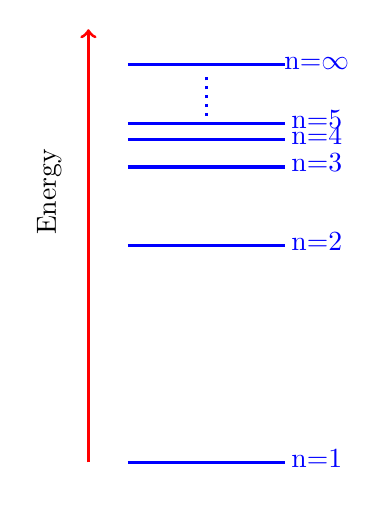
\begin{tikzpicture}[ scale=0.5, level/.style={very thick} ]
    \tikzset{rotdis/.style={->,decorate, draw=red,line width=0.4mm}}
                      \draw[level,blue] ( 6cm, 10.1cm) -- ( 10cm, 10.1cm)node[above,xshift=0.4cm, yshift=-0.2cm]{n=$\infty$};

                      \draw[level,blue, dotted] ( 8cm, 8.8cm) -- ( 8cm, 9.8cm) ;

              \draw[level,blue] ( 6cm, 8.6cm) -- ( 10cm, 8.6cm)node[above,xshift=0.4cm, yshift=-0.2cm]{n=5};

              \draw[level,blue] ( 6cm, 8.2cm) -- ( 10cm, 8.2cm)node[above,xshift=0.4cm, yshift=-0.2cm]{n=4};
          \draw[level,blue] ( 6cm, 7.5cm) -- ( 10cm, 7.5cm)node[above,xshift=0.4cm, yshift=-0.2cm]{n=3};
      \draw[level,blue] ( 6cm, 5.5cm) -- ( 10cm, 5.5cm)node[above,xshift=0.4cm, yshift=-0.2cm]{n=2};
    \draw[level,blue] ( 6cm, 0cm) -- ( 10cm, 0cm)node[above,xshift=0.4cm, yshift=-0.2cm]{n=1};
    \draw[rotdis]   (5cm,0cm) -- (5cm,11cm) node[right,midway, rotate=90, yshift=0.5cm]{Energy};
  \end{tikzpicture}
      \caption{The energy levels of hydrogen}
   \end{marginfigure}
\item[\docfilehook{Transition energies}{Transition energies}]
Bohr's models is able to explain the atomic spectrum of hydrogen. Each line in the spectrum represents a transition between two levels of energy. For example the line at 102nm represents the transition of an electron between the level three and the level one. The atomic spectrum of hydrogen is obtained by means of exciting hydrogen atoms with energy, so that the electron jumps from a lower level into a higher level. When the atom relaxes, it emits light as the electrons move back from high every levels into lower--more stable--levels. 






 \begin{figure}%%%%%%%MARGIN FIGURE
\begin{tikzpicture}[scale=0.7,
  >=stealth',
  pos=.8,
  photon/.style={decorate,decoration={snake,post length=1mm}}
]
\def\electron(#1,#2){%
    \fill[ball color=gray!30] (#1,#2) circle (5pt);
    \node at (#1,#2) {\texttt{-}};
}
\draw (0,0) [black, thick] circle [radius=1] node[above,xshift=-0.7cm, yshift=0.6cm]  {\large $n=1$} ;
\draw [black, thick] circle [radius=3] node[above,yshift=2.2cm]  {\large $n=2$} (0,4);
\draw [black, thick] circle [radius=4] node[above,yshift=2.9cm]  {\large $n=3$} (0,5);
\draw [->,photon, thick] (3.0, 0)--(1, 0) node[above,xshift=0.8cm]{$\Delta E_{2\rightarrow 1}$} ;
\draw [->,photon, thick] (2.8, 2.8) --(0, 1)node[above,xshift=2.7cm,yshift=1.2cm]{$\Delta E_{3\rightarrow 1}$} ;
\fill[black] (1,-4) rectangle (9,-6);
\draw [dashed, thick] (3.0, 0)--(3.7,-4);
\draw [dashed, thick] (2.8, 2.8)--(5.7,-4);
\fill[yellow] (3.7,-4) rectangle (3.8,-6) node[black,below,yshift=-0.2cm]{121nm} ;
\fill[yellow] (5.7,-4) rectangle (5.8,-6) node[black,below,yshift=-0.2cm]{102nm} ;
\electron(3.0, 0);
\electron(2.8, 2.8);
\end{tikzpicture}
    \caption{Representation of two energy transitions}   
 \end{figure}%%%%%%%MARGIN FIGURE
 

 
 
 
The energy for an electron transition between two energy levels, from $n_1$ to $n_1$ is given by:
\resizeableyellownote{2.5}{1}{Add this formula to your flashcard.}
\begin{equation*}
\boxed{  \Delta E_{n_2\rightarrow n_1}=-2.178\times 10^{-18} \Bigg( \frac{1}{n_2^2}-\frac{1}{n_1^2}\Bigg)  } \quad \textcolor{blue}{\text{Energy transition formula}}
\end{equation*}
where:
\begin{where}
 \item $\Delta E_{{n_2}\rightarrow n{_1}}$   is the energy in joules for the transition, the line in the spectra
 \item $n_2$  is the number of the final level
  \item $n_1$  is the number of the initial level
    \item $-2.178\times 10^{-18}J=R_H$  is called the Rydberg ($-13.59eV=R_H$)

\end{where}


\begin{example} %%%%%%%%%%%%%%%%%%%%%%%% EXAMPLE BOX
Calculate the following transition energies:
\begin{enumerate}[label=(\alph*)]
\item $\Delta E_{4\rightarrow 3}$ in J
\item $\Delta E_{4\rightarrow 3}$  in eV
\item Calculate the final energy level for a transition with energy 1.34eV knowing the first energy level involved in the transition is $n=3$
\end{enumerate}
\textlcsc{ \textcolor{dgreen}{\Large \textbf{Solution}} }\\
(a) We will use the energy transition formula to calculate the energy needed to move one electron from $n_1=4$ to $n_2=3$:
\begin{equation*}\begin{split}
\Delta E_{n_2\rightarrow n_1}=-13.59 \Bigg( \frac{1}{n_2^2}-\frac{1}{n_1^2}\Bigg)  =-13.59\Bigg( \frac{1}{3^2}-\frac{1}{4^2}\Bigg)\\
=-13.59\Bigg( 0.111- 0.0625 \Bigg)=-0.66eV
\end{split}\end{equation*}
The transition energy is negative, this means the atom releases energy when transitioning between these two levels.\\
(b) We will use the energy transition formula this time in eV:
\begin{equation*}\begin{split}
\Delta E_{n_2\rightarrow n_1}=-2.178\times 10^{-18} \Bigg( \frac{1}{n_2^2}-\frac{1}{n_1^2}\Bigg)  =-2.178\times 10^{-18}\Bigg( \frac{1}{3^2}-\frac{1}{4^2}\Bigg)\\
=-2.178\times 10^{-18}\Bigg( 0.111- 0.0625 \Bigg)=-1.058\times 10^{-19}J
\end{split}\end{equation*}
(c) In this case, we know $\Delta E_{n_2\rightarrow 3}$ and we know the initial level is $n_1=3$. We can certainly solve for $n_2$:
\begin{equation*}\begin{split}
1.34=-13.59 \Bigg( \frac{1}{n_2^2}-\frac{1}{3^2}\Bigg)  =-13.59\Bigg( \frac{1}{n_2^2}-\frac{1}{9}\Bigg)
\end{split}\end{equation*}
Solving for $n_2$ we have: $n_2=9$. Mind you need to square root $n_2^2$ to get the final value of $n_2$.\\
\faDiamond\ \textlcsc{ \textcolor{dgreen}{\Large \textbf{Study Check}} }\\
Calculate the following transition energies:
(a) $\Delta E_{9\rightarrow 3}$ in J and (b) $\Delta E_{5\rightarrow 4}$  in eV.
\flushright Answer: (a) $-2.15\times 10^{-19}J$; (b) -0.30eV.
\end{example}%%%%%%%%%%%%%%%%%%%%%%%% EXAMPLE BOX
\end{description}



\section{Quantum mechanics and electronic structure}
Bohr's model was a simplistic model. Still, it was able to correctly predict the fine structure of hydrogen--the atomic spectrum of hydrogen--with its energy transitions. The downside of this model resulted from considering that the electron moves in different orbits. The correct assumption of the model was that the energy levels of the atom were quantized--electrons can only exist in specific energy levels characterized by the number $n$ and not in a continuum of energy. This section will cover a more realistic theory that describe the structure of the atom: quantum mechanics. The outcome of this section is the existence of orbitals and quantum numbers.
\begin{marginfigure}
    \begin{shadequote}[l]{Schr\"{o}dinger}
The present is the only things that has no end.\end{shadequote}   
\end{marginfigure}
\sloppy
\begin{description}
\item[\docfilehook{Quantized energy and continuum energy}{Quantized energy and continuum energy}] 
Quantum mechanics is a theory used to do modeling in chemistry. Think of an engineer designing a plane. Before building and selling the plane engineers have to model it with computer software to make sure the plane will work properly. In a similar way, chemists carry modeling. The theory behind normal engineering modeling is classical mechanics, based in Newton's law.The theory behind chemistry modeling is quantum mechanics, based in Schr\"{o}dinger equation. Classical mechanics is based on the idea that the energy of a system, a plane or a car, is continuum, that is, the car or a plane can have any possible energy, starting from zero to any number you can think of. 
Differently, quantum mechanics is based in the idea that the energy of a system, an atom or a molecule, is quantized, that is the energy of an atom or a molecule can only be certain specific values. For example, a hydrogen atom can only have $E_1$, or  $E_4$ or $E_5$. It would never have a energy corresponding to $E_{\frac{1}{2}}$. That is the meaning of quantized.
\begin{marginfigure}
\begin{tikzpicture}
\begin{scope}[xshift=0cm]
\filldraw[even odd rule,inner color=red,outer color=red!5, draw=white] circle (1.0) node[below,yshift=2cm] {Representation of an electron};
\end{scope}
\begin{scope}[yshift=-4cm]
     \node[inner sep=0pt] (russell) at (0,0)
    {\includegraphics[width=.55\textwidth]{chapter3/figure1-8}} node[below,yshift=2cm] {Representation of a tennis ball};
       \end{scope}
\end{tikzpicture}
      \caption{An electron is a quantum object whereas a tennis ball is a classical object}
 \end{marginfigure}
 
\item[\docfilehook{The wave function}{The wave function}] 
In quantum mechanics the wave function of an atom or a molecule $\Psi$ is a complex function that contains all information of this atom or this molecule. By means of this function, we can simulate the behavior and properties of the atom. You want to think of $\Psi$ as a box that contains information, in particular all information of the system you want to simulate, such as a large molecule or a small atom. $\Psi$ depends on several variables, in particular the position and two angles; as such $\Psi$ results from the multiplication of an angular and radial function.This function has no real meaning and only its square value has a real physical interpretation. $\Psi^2$ represents the probability of finding an electron near a particular point in space. In order to calculate any property of the system of interest, we need to solve Schr\"{o}dinger's equation:
\begin{equation*}\begin{split}
\hat{H}\Psi=E\Psi
\end{split}\end{equation*}
$\hat{H}$ is called Hamiltonian operator and depends on the kinetic and potential energy of the system.
\item[\docfilehook{Orbitals}{Orbitals}] 
An orbital is a single-electron wave function. In another words is a wave function that contains information of a single electron. The square value of an orbital represents the probability of finding an electron at a specific location. Electrons are very different than larger objects such as for example a tennis ball. Larger objects are localized, that is they are located at a specific point in space. Differently, electrons are delocalized, that means they are not located at a single point in space and time, and therefore we can only guess the probability of finding the electron an a specific point.
\item[\docfilehook{Different types of orbitals}{Different types of orbitals}] 
There are four different types of orbitals: \begin{it}s\end{it} orbitals, \begin{it}p\end{it} orbitals, \begin{it}d\end{it} orbitals and \begin{it}f\end{it} orbitals. At the same time, there are one type of \begin{it}s\end{it} orbitals, three types of \begin{it}p\end{it} orbitals ($p_x$, $p_y$ and $p_z$) and five types of \begin{it}d\end{it} orbitals ($d_{xy}$, $d_{xz}$, $d_{yz}$, $d_{z^2}$ and $d_{x^2-y^2}$). For example, \begin{it}s\end{it} orbitals are very easy to visualize and they look like spheres. Differently, \begin{it}p\end{it} orbitals are more complex. To understand their shape, image you hold a ballon with both of your hands and you twist it in different directions.
 
\begin{figure}%%%%%%%MARGIN FIGURE
%      \includegraphics[width=1\linewidth,scale=0.2]{chapter3/figure1-6}
%\label{image3.5}
%      \caption{Shape of the different orbitals.}
 
  \centering
  \begin{tikzpicture}
  
 \begin{scope}[font=\itshape]% to not type it every time, but better go for math mode
      \draw[-latex] (0,0)--(1,0) node[above]{x};
  \draw[-latex] (0,0)--(-.5,-0.7) node[above]{y};
  \draw[-latex] (0,0)--(0,1) node[above]{z};
\orbital[scale = 1.5, pos = {(0,0)}]{s}
  \node[above] at (0.7,0.7) {s};
 
 
    \end{scope}
    \node[minimum width=\columnwidth] at (current bounding box.center){};  
    \end{tikzpicture}

  
 \begin{tikzpicture}
  \begin{scope}[font=\itshape]% to not type it every time, but better go for math mode
 \draw[-latex] (0,0)--(1,0) node[above]{x};
  \draw[-latex] (0,0)--(-0.5,-0.7) node[above]{y};
  \draw[-latex] (0,0)--(0,1) node[above]{z};
  \orbital[pos = {(0,0)}]{py}
  \node[above] at (0.7,0.7) {p$_x$};


  \draw[-latex] (3,0)--(4,0) node[above]{x};
  \draw[-latex] (3,0)--(2.5,-0.7) node[above]{y};
  \draw[-latex] (3,0)--(3,1) node[above]{z};
  \orbital[pos = {(3,0)}]{px}
  \node[above] at (3.7,0.7) {p$_y$};

  \draw[-latex] (6,0)--(7,0) node[above]{x};
  \draw[-latex] (6,0)--(5.5,-0.7) node[above]{y};
  \draw[-latex] (6,0)--(6,1) node[above]{z};
  \orbital[pos = {(6,0)}]{pz}
  \node[above] at (6.7,0.7) {p$_z$};
  

  
  \end{scope}
    \node[minimum width=\columnwidth] at (current bounding box.center){};  
    \end{tikzpicture}
      \begin{tikzpicture}
  \begin{scope}[font=\itshape]% to not type it every time, but better go for math mode
  \draw[-latex] (0,0)--(1,0) node[above]{x};
  \draw[-latex] (0,0)--(-0.5,-0.7) node[below]{y};
  \draw[-latex] (0,0)--(0,1) node[above]{z};
\orbital[pos = {(0,0)}]{dxy}
  \node[above] at (0.7,0.7) {d$_{xy}$};



  \draw[-latex] (3,0)--(4,0) node[above]{x};
  \draw[-latex] (3,0)--(2.5,-0.7) node[below]{y};
  \draw[-latex] (3,0)--(3,1) node[above]{z};
\orbital[pos = {(3,0)}]{dxz}
  \node[above] at (3.7,0.7) {d$_{yz}$};

  \draw[-latex] (6,0)--(7,0) node[above]{x};
  \draw[-latex] (6,0)--(5.5,-0.7) node[below]{y};
  \draw[-latex] (6,0)--(6,1) node[above]{z};
  \orbital[pos = {(6,0)}]{dyz}
  \node[above] at (6.7,0.7) {d$_{xz}$};
  
     \draw[-latex] (9,0)--(10,0) node[above]{x};
  \draw[-latex] (9,0)--(8.5,-0.7) node[below]{y};
  \draw[-latex] (9,0)--(9,1) node[above]{z};
\orbital[scale = 1.0, pos = {(9,0)}]{dx2y2}
  \node[above] at (9.7,0.7) {d$_{x^2-y^2}$};
  \end{scope}
    \node[minimum width=\columnwidth] at (current bounding box.center){};  
    \end{tikzpicture}
    
         \begin{tikzpicture}
  \begin{scope}[font=\itshape]% to not type it every time, but better go for math mode
  \draw[-latex] (0,0)--(1,0) node[above]{x};
  \draw[-latex] (0,0)--(-0.5,-0.7) node[below]{y};
  \draw[-latex] (0,0)--(0,1) node[above]{z};
\orbital[pos = {(0,0)}]{dz2}
  \node[above] at (0.7,0.7) {d$_{z^2}$};
   \end{scope}
    \node[minimum width=\columnwidth] at (current bounding box.center){};  

      \end{tikzpicture}

    \caption{$s$, $p$ and $d$ orbitals. $s$ orbitals have spherical symmetry, whereas $p$ orbitals have two lobes with dumbbell shape, a positive and negative lobe. The name for the different $p$ orbitals depend on the axis that it crosses. For example, $p_x$ orbitals cross the x axis. The positive part of this orbital corresponds with the positive part of the axis--the right side. $d$ orbitals have more complex shapes. Most of $d$ orbitals have four lobes, two positive and two negative. For example, orbital $d_{xy}$ is placed in the xy plane without crossing any axis. Differently, orbital $d_{x^2-y^2}$ is located in the xy plane and cross both axis. The blue part of the orbital represent the positive side of the orbital, whereas the grey part is negative.}   

 \end{figure}%%%%%%%MARGIN FIGURE




 
\end{description}



\section{Electronic configuration of an atom}
Atoms have in general many electrons. These electrons are arranged in the atom in a very specific way creating what we know as electronic structure. You want to think about the electronic configuration of an atom as a code that tells you the orbital location of each electron in the atom. On the other hand, there are two ways to present electronic configurations. One is called full electronic configuration (for example $1s^22s^1$) and the other one is called condensed electronic configuration (for example $[He]2s^1$). The full configuration display all orbitals in an atom, whereas the abbreviated only display the valence electrons--these electrons are less-tied to the nucleus--and the core has nobel. At the same time, every orbital is characterized by a set of numbers--these are called quantum numbers. These numbers are not independent from each other and there are constrictions that relate the possible values of the quantum numbers. This section will show you how to construct electron configurations and how to extract quantum numbers from it.
\sloppy
\begin{description}
\item[\docfilehook{Electron energy levels}{Electron energy levels}] 
The electrons in an atom are arranged in different energy levels. Some levels have lower energy and the electron in these levels are close to the nucleus being also strongly attached to it, whereas other levels have higher energy and the electrons in these levels are less attached to the nucleus. Still, each electron in an energy level have the same energy. The energy levels are labeled with a number $n$ that equals to a single number such as 1, 2, 3 and so on. The first energy level is $n=1$ and never $n=0$--think of this as an apartment in a building, the first floor is flour one. For example all electrons in level one $n=1$ have the same energy. There is a limit to the number of electrons in an energy level and we call this occupancy. Only a few electrons can occupy the lower energy levels, while more electrons can be accommodated in higher energy levels.  Level one can only fit two electrons, whereas level two can fit a total number of eight electrons. The maximum number of electrons allowed in any energy level is calculated using the formula 

\begin{marginfigure}[0cm]%%%%%%%MARGIN FIGURE
\begin{tcolorbox}[tab2,tabularx={X|X}]%%%% FANCY COLOR TABLE
 l value     &  Orbital label\\\hline\hline
0  &  $s$       \\\hline
1  &   $p$        \\\hline
2  &   $d$       \\\hline
3  &  $f$       
\end{tcolorbox}%%%% FANCY COLOR TABLE
 \end{marginfigure}%%%%%%%MARGIN FIGURE


\begin{marginfigure}[0cm]%%%%%%%MARGIN FIGURE
\begin{tcolorbox}[tab2,tabularx={>{\hsize=.4\hsize}X|X}]%%%% FANCY COLOR TABLE
Quantum number   &  Values\\\hline\hline
$n$  &  1, 2, 3...       \\\hline
$l$  &   0, 1, ..., n-1        \\\hline
$m_l$  &   -l, -l+1, ..., 0, ..., l-1, l       \\\hline
$m_s$  &  $+^1/_2$ or $-^1/_2$       
\end{tcolorbox}%%%% FANCY COLOR TABLE
 \end{marginfigure}%%%%%%%MARGIN FIGURE

\begin{marginfigure}[0cm]%%%%%%%MARGIN FIGURE
\begin{tcolorbox}[tab2,tabularx={X|X}]%%%% FANCY COLOR TABLE
 Orbital     &  Maximum Number of electrons  \\\hline\hline
    $s$  & 2    \\\hline
   $p$  &6      \\\hline
   $d$ &10      \\\hline
  $f$  &  14   
\end{tcolorbox}%%%% FANCY COLOR TABLE
 \end{marginfigure}%%%%%%%MARGIN FIGURE
 


\begin{equation}
2n^2 
\end{equation}
in which $n$ is the energy level. You can see by using this formula that for example, the third level can accommodate 27 electrons.


\begin{example} %%%%%%% EXAMPLE BOX with explanation
How many electrons can you fit in the energy level n=3.\\
\textlcsc{ \textcolor{dgreen}{\Large Solution} }\\
We will use the formula $2n^2 $ that gives the number of electrons that fit in a energy level $n$. As $n=3$, we can fit 18 electrons in this level. Remember, the larger the energy level the more electrons we can fit. \\
\faDiamond\ \textlcsc{ \textcolor{dgreen}{\Large \textbf{Study Check}} }\\At a given energy level you can fit 162 electrons. Identify the energy level.
\flushright Answer: $n=9$. 
\end{example}%%%%%%% EXAMPLE BOX with explanation



\item[\docfilehook{Sublevels}{Sublevels}] 
Each energy level consists of one or more sublevels, which contain electrons with identical energy. The number of sublevels in each level corresponds to $n$. For example, in the first energy level ($n=1$) we have only one sublevel, whereas in the third energy level ($n=3$) we have three sublevels.
\begin{marginfigure}%%%%%%%MARGIN FIGURE
      \includegraphics[width=1\linewidth,scale=0.5]{chapter3/figure1-4}
      \caption{Table indicating the orbital filling order. In order to use this table you need to start by filling the orbital $1s$, after that you follow the arrow until next level and start from the begining of next arrow. For example, after $3d$ you need to fill $6s$.}
      \label{orbitalfill}
\end{marginfigure}%%%%%%%MARGIN FIGURE
\item[\docfilehook{Orbital Filling}{Orbital Filling}] 
Atoms in general contain numerous orbitals and each orbital should be filled with electrons. In every orbital you can fill only a maximum number of electrons. For example, in a $s$ orbital you can put a maximum of two electrons. That is why you will find $s^1$ orbitals and $s^2$, with the latest being completely filled with electrons. In a $p$ orbital you can put a maximum of six electrons and in a $d$ orbital a maximum of ten. Finally, in a $d$ orbital you can put fourteen or less electrons. For example, the orbital notation $p^2$ is correct as in $p$ orbitals you can put six or less electrons. In this case, this orbital still have space to accept more electrons. Differently, the notation $d^12$ is incorrect, as in $d$ orbitals you can fit ten or less electrons and never twelve.

In order to fill the orbitals you should follow Figure \ref{orbitalfill}. You start from the top of the table and follow the arrows that indicates the orbitals ordering. For examples the first orbital to be filled will be $1s$. After that you should fill  $2s$ and  $2p$. After that you should fill $3s$, $3p$, $4s$, $3d$, and $4p$. There is a maximum number of electrons that can occupy each orbital. An s orbital holds a maximum of 2 electrons. A p orbital takes up to 6 electrons, a d orbital can hold up to 10 electrons, and an f orbital holds a maximum of 14 electrons. An orbital can be completely filled with electrons, partially filled or empty. For example a $3s^1$ is half-filled with one electrons and $2p^6$ is completely filled. Another example, a $3d$ orbital is empty and can accommodate a maximum of 10 electrons.

\item[\docfilehook{Full electron Configuration}{Full electron Configuration}] The full electron configuration of an atom is obtained by placing the total number of electrons of the atom in different orbitals with increasing energy. For example, the electron configuration for helium is written as $1s^2$ and the one for Li is $1s^2 2s^1$.  First, how do we know the total number of electrons in an atom? That is the same as the atomic number and is indicated in the periodic table. Look for the element and the atomic number is on the top left side of the element. For example, the atomic number of hydrogen is one, and the number of electrons in He is two. Similarly, nitrogen has seven electrons. Second, how do we know what orbitals to fill? Figure \ref{orbitalfill} shows the orbital order. You need to start from the top of the image, from orbital $1s$ and proceed to next arrow, starting from the end of the arrow. This way, after $1s$ goes $2s$ and then $2p$, $3s$, $3p$, $4s$, and $3d$. Mind that every $s$ orbital can only fit two electrons, and $p$ orbitals can fit six electrons, and so on. The following example will help you construct the electron configuration for a given atom.




\begin{example} %%%%%%% EXAMPLE BOX with explanation
Obtain the electronic configuration of C.\\
\textlcsc{ \textcolor{dgreen}{\Large Solution} }\\
The atomic number of C is Z=6 and that means C has 6 electrons. The orbital order from Figure \ref{orbitalfill} is: $1s$,$2s$, $2p$, $3s$, etc. Each $s$ orbital can fit two electrons, whereas the occupancy of  the $p$ orbitals is six electrons. Hence the electronic configuration of C is: $1s^2 2s^2 2p^2$. The $s$ orbitals are all filled, whereas the $p$ orbital is only occupied with two electrons.
\\
\faDiamond\ \textlcsc{ \textcolor{dgreen}{\Large \textbf{Study Check}} }\\Obtain the electronic configuration of Ni.
\flushright Answer: $1s^2 2s^2 2p^6 3s^2 3p^6 4s^2 3d^8$. 
\end{example}%%%%%%% EXAMPLE BOX with explanation


\item[\docfilehook{Abbreviated Electron Configuration}{Abbreviated Electron Configuration}] The electronic configuration of Nickel (Ni) is  $1s^2 2s^2 2p^6 3s^2 3p^6 4s^2 3d^8$, whereas the electronic configuration of Argon (Ar) is  $1s^2 2s^2 2p^6 3s^2 3p^6 $. If you look closely, the electronic configuration of Argon is part of the electronic configuration of Nickel. We called both of these configuration the \emph{full electronic configuration}. We can make the configuration of Nickel shorter by writing the electronic configuration of Nickel as: $[Ar]4s^2 3d^8$. We call this last configuration as the \emph{abbreviated electronic configuration}. You can figure out faster the abbreviated electronic configuration by looking for the noble gas on the table on the row above the element, and the period (row on the table) of the element. Ni is located in the period number four and the noble gas above this period is Ar. At the same time Ar has 18 electrons. That will give you the core $[Ar]$ with 18 electrons, and the remaining 10 electrons (Ni has 28 electrons) starting by the orbital $4s$, according to the period four. The electrons in the noble gas core are called \emph{core electrons}, whereas the rest of the electrons are known as \emph{valence electrons}. For the case of Ni, it has 18 core electrons in the Ar core and 10 electrons in the valence.\\
Let us work another example: Cd. It has 48 electrons, and is located in group 5. The novel gas on the group above is Kr with 36 electrons. The core will be Kr--the novel gas on the period above--and we start right away filling $5s$ electrons--Cd belong to period five. In the valence electrons, we will place 12 electrons. Hence, the abbreviated configuration will be: $[Kr]5s^{2}4d^{10}$. 


\begin{example} %%%%%%% EXAMPLE BOX with explanation
Obtain the full and abbreviated electronic configuration of Silver (Ag, Z=47).\\
\textlcsc{ \textcolor{dgreen}{\Large Solution} }\\
The atomic number of Ag is Z=47 and that means Nb has 47 electrons. The orbital order from Figure \ref{orbitalfill} is: $1s$,$2s$, $2p$, $3s$, etc. Each $s$ orbital can fit two electrons, whereas the occupancy of  the $p$ orbitals is six electrons. $d$ orbitals can fit 10 electrons. Hence the full electronic configuration of Ag is: 
$1s^2 2s^2 2p^6 3s^2 3p^6 3d^{10} 4s^2 4p^6 4d^{10} 5s^1$. As Kr is the noble gas on top with 36 electrons, the abbreviated electronic configuration of Ag is: $[Kr] 4d^{10} 5s^1$. Ag has 36 core electrons and 11 valence elenctrons.
\\
\faDiamond\ \textlcsc{ \textcolor{dgreen}{\Large \textbf{Study Check}} }\\
Obtain the abbreviated electronic configuration of Cobalt (Co, Z=27).
\flushright Answer: $ [Ar] 3d^7 4s^2$. 
\end{example}
\begin{marginfigure}
\end{marginfigure}%%%%%%% EXAMPLE BOX with explanation


\item[\docfilehook{Orbital diagrams}{}] orbital diagrams are a visual way to represent the electron configuration of an atom. Every $s$ orbital is represented by a box that can fix two electrons. Differently, $p$ orbitals are composed of three boxes--$p_x$, $p_y$ and $p_z$--with a total capacity of six electrons, with two electrons per box. $d$ orbitals are represented by five boxes with a total capacity of ten electrons. Only the valence electrons are normally represented.


\begin{MOdiagram}[style=round,AO-width
=15pt, distance=1.5cm,lines={none},names-style={anchor=left, draw=blue}]
 \AO(3cm){s}{0;pair}\node[right,xshift=4mm] at (-0.7,0) {\Large s};
 \end{MOdiagram}\\
\begin{MOdiagram}[style=round,AO-width
=15pt, distance=1.5cm,lines={none},names-style={anchor=left, draw=blue}]
 \AO(3cm){p}{0;pair, pair, pair} \node[right,xshift=4mm] at (-0.7,0) {\Large p};
 \end{MOdiagram}\\
\begin{MOdiagram}[style=round,AO-width
=15pt, distance=1.5cm,lines={none},names-style={anchor=left, draw=blue}]
 \AO(3cm){p}{0;pair, pair, pair}  \AO(6cm){s}{0;pair}\AO(7cm){s}{0;pair} \node[right,xshift=4mm] at (-0.7,0) {\Large d};
 \end{MOdiagram}
\begin{example} %%%%%%% EXAMPLE BOX with explanation
Obtain the orbital diagram for oxygen given the electron configuration: $[He] 2s^2 2p^4$\\
\textlcsc{ \textcolor{dgreen}{\Large Solution} }\\
The orbital diagram should include an s orbital and  a p orbital. The $s$ orbital contains a single box, whereas the p orbital contain three different boxes. The $s$ orbital is fully occupied with two electrons, whereas the $p$ orbital contain four electrons. The first three $p$ electron will occupy separate boxes while the fourth electron will occupy the first box with opposite spin.
\begin{MOdiagram}[style=round,AO-width
=15pt, distance=1.5cm,lines={none},names-style={anchor=left, draw=blue}]
% \atom[]{left} { 2s = {0;up}  }
% \atom[]{right}{ 2p = {0;up} }
 \AO(3cm){s}{0;pair}
  \AO(4.5cm){p}{0;pair, up, up}
\node[right,xshift=4mm] at (-0.7,0) {\Large O $[He] 2s^2 2p^4$};
\node[below left=2mm and -6mm of AO1]  {\Large 2s};
\node[below left=2mm and -30mm of AO1]  {\Large 2p};
 \end{MOdiagram}
\\
\faDiamond\ \textlcsc{ \textcolor{dgreen}{\Large \textbf{Study Check}} }\\
Obtain the orbital diagram for Li given the electron configuration: $[He] 2s^1$.\
\flushright Answer: \begin{MOdiagram}[style=round,AO-width
=15pt, distance=1.5cm,lines={none},names-style={anchor=left, draw=blue}]
% \atom[]{left} { 2s = {0;up}  }
% \atom[]{right}{ 2p = {0;up} }
 \AO(3cm){s}{0;up}
 \end{MOdiagram}
\end{example}
\begin{marginfigure}
\end{marginfigure}%%%%%%% EXAMPLE BOX with explanation

 \item[\docfilehook{Quantum numbers}{Quantum numbers}] Every electron in an orbital is characterized by four different quantum numbers. Each electron in an atom has unique values for these quantum numbers. The first quantum number $n$ is called \emph{principal quantum number} and has integral values such as 1, 2 or 4. $n$ cannot be zero. The second quantum number $l$ is called \emph{angular quantum number} and has integral values such as 1, 0 or 4. $l$ can be zero and the values of $l$ depend on the values of $n$. In particular $l$ goes from $0$ until $n-1$. For example if $n=3$, therefore $l$ can vary be: $0, 1, 2$. The third quantum number $m_l$ is called \emph{magnetic quantum number} and has integral values that vary from  $-l$, $-l-1$, ..., 0, ..., $l+1$, $l$. For example, if $l=3$, $m_l$ can be any of these values: -3, -2, -1, 0, 1, 2, or 3. The fourth quantum number $m_s$ is called \emph{spin quantum number} and can only be either $+^1/_2$ or $-^1/_2$. Two of the quantum numbers can be extracted from the orbital label. For example
\end{description}


\begin{example} %%%%%%%%%%%%%%%%%%%%%%%% EXAMPLE BOX
Indicate if the following combination of quantum numbers is allowed:
\begin{tabularx}{\textwidth}{
    >{\centering}m{.185\linewidth} 
    *{4}{Y} }
  \toprule
\heading{$n$} & \heading{$l$}  &  \heading{$m_1$} & \heading{$m_s$} & \heading{Allowed?}   \\
    \midrule
  1	&	1	&	0	&	$+^1/_2$    \\
   2	&	0&		0	&	$+^1/_2$   \\
3		&3	&	-1	&	$-^1/_2$\\    
    \bottomrule
\end{tabularx}
\textlcsc{ \textcolor{dgreen}{\Large \textbf{Solution}} }\\
The four quantum numbers are not independent. The quantum number $n$ is related to the quantum number $l$ and the number $l$ is related to $m_l$. The only quantum number that is independent is the spin, $m_s$ which can be $+^1/_2$ or $-^1/_2$. The first combination is not possible, as if $n=1$, $l$ can only be $n-1$, that is zero. The second combination is correct, as if $n=2$, the number $l$ can be: 0 or 1. At the same time if $l=0$, then $m_l$ can also be zero. And finally, the spin value of $+^1/_2$ is allowed. The last combination is not allowed, as $n$ and $l$ cannot be the same number.
\begin{tabularx}{\textwidth}{
    >{\centering}m{.185\linewidth} 
    *{4}{Y} }
  \toprule
\heading{$n$} & \heading{$l$}  &  \heading{$m_1$} & \heading{$m_s$} & \heading{Allowed?}   \\
    \midrule
  1	&	1	&	0	&	$+^1/_2$ & No   \\
   2	&	0&		0	&	$+^1/_2$ & Yes   \\
3		&3	&	-1	&	$-^1/_2$&No\\    
    \bottomrule
\end{tabularx}
\faDiamond\ \textlcsc{ \textcolor{dgreen}{\Large \textbf{Study Check}} }\\
Indicate if the following combination of quantum numbers is allowed:
\begin{tabularx}{\textwidth}{
    >{\centering}m{.185\linewidth} 
    *{4}{Y} }
  \toprule
\heading{$n$} & \heading{$l$}  &  \heading{$m_1$} & \heading{$m_s$} & \heading{Allowed?}   \\
    \midrule
 4		&3&		3	&	$+^1/_2$    \\
  4		&3	&	3	&	$0$   \\
2		&1	&	-1	&	$+^1/_2$\\    
    \bottomrule
\end{tabularx}
\flushright Answer: yes, no, yes. 
\end{example}%%%%%%%%%%%%%%%%%%%%%%%% EXAMPLE BOX




\section{Periodic Trends}
Some atomic properties are periodic, which means that they follow a certain trends in the periodic table. These properties increases or decreases across a period and then the trend is repeated again in each successive period or group. We will consider here four atomic properties: the atomic size, the ionization energy, the metallic character and the electronegativity.

\sloppy
\begin{description}
\item[\docfilehook{Atomic Size}{Atomic Size}] The \emph{atomic radius} is the distance from the nucleus to the valence electrons. The atomic radius increases when going down a group in the periodic table (the columns of the table) and when going from right to left on the periodic table (in a period). For example, if we compare the atomic size of H and He, as He is further right it has a smaller radius ($r_{He}<r_{H}$). Similarly, if we compare H and Li, as Li is further down it will have a larger radius ($r_{H}<r_{Li}$).

\item[\docfilehook{Ionization Energy}{ Ionization Energy}] The \emph{ionization energy} (IE) is the energy needed to remove an electron from an atom in gas state. The ionization energy increases (this means more energy is needed to remove an electron) going up a group and when going across a period from left to right. In general, the ionization energy is low for the metals and high for the nonmetals. For example, if we compare the IE for H and He, as He is further right in the same period, it will have a larger IE and more energy will be needed to remove an electron ($IE_{H}<IE_{He}$). For the case of Li and H, the EI will be higher for H as it is further up in the same group ($IE_{H}>IE_{Li}$).
The ionization energy of hydrogen is  313Kcal:
\begin{center}\ce{ H_{(g)} -> H+_{(g)} + e-   + 313Kcal} \end{center}


\item[\docfilehook{Metallic character }{Metallic character }] 
All elements in the periodic table have somehow a certain \emph{metallic character} as they all can loose electrons as metals do--that is why metals are good conductors. The elements in the left part of the table are metals with a strong metallic character. Still, the elements in the right side of the table also have a certain metallic character (MC). The metallic character increases (the atom is more metallic) when going down a group (column) of the table and when going across a period (row) from right to left. For example, comparing K and Ca, we have that K is more metallic than Ca, as it is located further to the left in the same column ($MC_{K}>MC_{Ca}$). For the case of F and Cl, Cl is more metallic as it is located further down a group ($MC_{Cl}>MC_{F}$). 


\item[\docfilehook{Electronegativity}{Electronegativity}] 
Atoms combine with each other and  by sharing or give away electrons. The \emph{electronegativity} of an atom is its ability to attract the shared electrons when combined. Imagine two people holding a pillow with their hands, with the pillow representing a pair of electrons. If one of the person is more electronegative it will pull the pillow closer to them--it will attract more the electrons. Electronegativity (EN) increase (the atom is more electronegative) when going up a group (column) of the table and when going across a period (row), from left to right of the table. When comparing the EN of I and F, we found that F is more electronegative as it is further up in the same group ($EN_{F}>EN_{I}$). 
\begin{marginfigure}%%%%%%%MARGIN FIGURE
   \includegraphics[width=1\linewidth,scale=0.25]{chapter3/figure1-7}
\caption{Periodic properties across the table}
\end{marginfigure}%%%%%%%MARGIN FIGURE
\begin{example} %%%%%%%%%%%%%%%%%%%%%%%% EXAMPLE BOX
Compare the following property for the given couple of elements:
\begin{enumerate}[label=(\alph*)]
\item Atomic radius of N and F.
\item Ionization energy of Na and Cs.
\item Electronegativity of F and I.
\item Metallic character of N and F. 
\end{enumerate}
\textlcsc{ \textcolor{dgreen}{\Large \textbf{Solution}} }\\
(a) You go from N to F by moving from left to right on a row of the periodic table, hence the radius of N is larger than the radius of F. This is because the atomic radius decreases from left to right on a row.
(b) You go from Na to Cs by moving from up to down on a column of the periodic table, hence the ionization energy of Na is larger than for Cs. This is because the ionization energy decreases from top to bottom on a period.
(c) You go from F to I by moving from down to up on a column of the periodic table, hence the electronegativity of F is larger than for I. This is because the electronegativity energy increased from bottom to top on a period.
(d) You go from N to F by moving from left to right on a row of the periodic table, hence the metallic character of N is larger than for F. This is because the metallic character increased from right to left on a period.
\\
\faDiamond\ \textlcsc{ \textcolor{dgreen}{\Large \textbf{Study Check}} }\\
Compare the following property for the given couple of elements:
\begin{enumerate}[label=(\alph*)]
\item Atomic radius of F and I.
\item Electronegativity of Cs and Na.
\end{enumerate}
\flushright Answer: (a) radius I > F; (b) Electronegativity Na > Cs.
\end{example}%%%%%%%%%%%%%%%%%%%%%%%% EXAMPLE BOX

\item[\docfilehook{Electron affinity}{}] 
The electron affinity (EA) is the tendency of an atom to receive one or more electrons becoming negatively charged.  Electron affinities are positive values and the larger this value the larger the tendency of the atom to accept electrons. For example, the electron affinity of hydrogen is 17Kcal:
\begin{center}\ce{ H_{(g)} + e-   +17Kcal -> H^{-}_{(g)} } \end{center}
EA increases from left to right in a given period, that means the elements from the right of the table are more willing to gain electrons becoming negatively charged.

\end{description}









\end{document}
%\textquotesingle

%\section{The atom}\marginnote{ \faEnvelope\myemail{dtorresrangel@bmcc.cuny.edu}{Error in the Book}{ Send Me typos!}}
%XXXXX
%\sloppy
%\begin{description}
%\item[\docfilehook{Elements and Symbols}{Elements and Symbols}] 
%\end{description}
%

%\begin{marginfigure}%%%%%%%QUOTES
%    \begin{shadequote}[l]{Democritus}
%Nothing exists except atoms and empty space; everything else is opinion.
%\end{shadequote}   \end{marginfigure}%%%%%%QUOTES
%\begin{marginfigure}%%%%%%%MARGIN FIGURE
%      \includegraphics{chapter3/figure1}
%      \label{fig:marginfig}
%   \end{marginfigure}%%%%%%%MARGIN FIGURE

%\begin{definition}[Political Factors]%%%%%%%%%ADITIONAL INFO BOX
%\begin{minipage}{0.25\linewidth}
%\includegraphics[width = \linewidth]{example-image-a}
%\end{minipage}%
%\hfill
%\begin{minipage}{0.7\linewidth}
%Analyses to what degree the government intervenes in the
%economy. It includes regulations and legal issues and defines
%both formal and informal rules under which the firm must
%operate. Political factors include: tax policy, employment laws,
%environmental regulations, trade restriction tariffs and political
%stability.
%\end{minipage}%
%\end{definition}%%%%%%%%%ADITIONAL INFO BOX
%
%\begin{example} %%%%%%% EXAMPLE BOX with explanation
%Obtain the electronic configuration of C.\\
%\textlcsc{ \textcolor{dgreen}{\Large Solution} }\\
%The atomic number of C is Z=6 and that means C has 6 electrons. The orbital order from Figure \ref{fig:orbitaltable} is: $1s$,$2s$, $2p$, $3s$, etc. Each $s$ orbital can fit two electrons, whereas the occupancy of  the $p$ orbitals is six electrons. Hence the electronic configuration of C is: $1s^2 2s^2 2p^2$. The $s$ orbitals are all filled, whereas the $p$ orbital is only occupied with two electrons.
%\\
%\faDiamond\ \textlcsc{ \textcolor{dgreen}{\Large \textbf{Study Check}} }\\Obtain the electronic configuration of Ni.
%\flushright Answer: $1s^2 2s^2 2p^6 3s^2 3p^6 4s^2 3d^8$. 
%\end{example}
%\begin{marginfigure}
%\begin{work} % 
%\textlcsc{ \textcolor{olive}{\Large Get the Answer by: } }
%\begin{enumerate}
%\item Get the electrons
%\item Check the orbital order table
%\item Fill each orbital following the order
%\end{enumerate}
%\end{work}% 
%\end{marginfigure}%%%%%%% EXAMPLE BOX with explanation


%Table \ref{tab:units} % TABLE OR FIGURE REFERENCE
